\section{Results: Connecting CTC to Computation} 

\begin{figure}[t]
\centering

\includegraphics[width=\textwidth]{figures/ctc_figure.pdf}
\caption{\emph{Cross-task scaling of full vs.\ chunked attention (with mask mixing )} We include average chunked and full attention performance at different contexts on our task suite, as well as several task-specific examplars on some high-CTC tasks. High-\cname tasks are more challenging for both methods, and correspond to growing gaps on larger corpora. Relative trends hold even on exemplars. } 
\label{fig:multitask_fig4}
\end{figure}


\subsection{Experimental Setup}

Our \cname definition suggests that higher-\cname tasks' computational requirements scale much more rapidly on larger corpora, but how do we measure this? To isolate performance of models within architectural constraints, \emph{our experiments focus on task-specific in-domain fine-tuning}. By varying across different model scales and attention approaches (especially standard vs chunked attention), we measure the ``best possible'' task performance at different levels of computation, and can consequently draw conclusions about where more or less computation is necessary.

We train several models (primarily Qwen3.5-4B, the most performant open-weight model of its scale we could find at time of writing) with full-fine-tuning (note LoRA may also be effective, Appendix~TODO), with a learning rate of 5e-5 which we find empirically effective. Note that Qwen3.5 models use 75\% GDN layers, which are already linear, so we only apply chunked attention to full attention layers. We also by default always enable mask mixing (anneal from $p=0.8$ to $p=0$ over training) for chunked training.

We use existing or i.i.d generated train sets where applicable, though for the OBLiQ twitter setting we generate our own synthetic train data as there's no standard train set (TODO details). Unless otherwise specified, we'll always train for 1 epoch on 20k datapoints per task, with evenly split examples across context lengths of 2k, 4k, 8k, 16k and 32k (matching the corpus sizes we evaluate on). For all our tasks, we pass corpora into LCLMs with a prompt format as below (bolded parts indicate generations at test-time):

% \prasannnote{TODO more descriptive section names}
% \sewonnote{Is this section about validating \cname? Rather, I think it's about connecting task complexity (\cname) and model complexity.}

% We here walk through our design decisions with a motivating task. We'll show how architectural decisions interact with task structure and scale, before getting into our main results (Section~\ref{sec:taskcompresults}). 

% We previously investigated how improving learning dynamics can be helpful for different approaches on higher \cname tasks, especially with mask mixing. This isolates the role of learning signal, \textit{but does this overcome architectural limitations of chunked attention}? We measure performance over increasing corpus sizes to connect \cname and method complexity.


{\small$${\texttt{[Initial]\textcolor{jacobcolor}{\textit{ 1:[Doc 1 content] \ldots N:[Doc N content]}} [Query] \textbf{[Answer]}}}$$}



%We report in Table~\ref{tab:mask-mix-suite} an exemplar set of settings where, when comparing the inclusion vs the exclusion of mask mixing, we see notable gains. Overall, mask mixing seems to be a consistent trick to aid learning in our settings: allowing for better performance with higher inference-scalability. .



% That said, \emph{following our application of mask mixing to our main results} (Figure~\ref{fig:sec5-cross-task}), we note that the fundamental gap from \cname remains even with mask mixing, suggesting that while learning signal issues can be addressed via analysis of learning dynamics, addressing gaps in complexity is a longer-term problem. 





% \sewonnote{Setup is mixed in this section. Clearly separate the setup to the earlier section, so that this section can solely focus on results.}
\subsection{Main Results}

\paragraph{All Methods, Particularly Chunked Attention, Scale Much Worse on High-\cname Tasks} We plot in figure figure~\ref{fig:multitask_fig4} an average of full attention (solid lines) and chunked attention (dashed lines) performance for all High-\cname and Low-\cname tasks across \bench{}. Note how the gap between solid lines and dashes lines grow larger at larger contexts. \claude{Both effects are visible in the class averages. Full attention itself degrades roughly twice as fast on the high-\cname{} side: from 2k to 32k the low-\cname{} average falls $0.910 \rightarrow 0.788$ (retaining 87\% of its 2k score) while the high-\cname{} average falls $0.851 \rightarrow 0.511$ (retaining 60\%). Chunked attention then adds a second, much larger penalty that is almost entirely confined to the high-\cname{} side: it recovers 98.8\% of full-attention performance at 2k and 98.7\% at 32k on low-\cname{} tasks (an absolute gap of $0.011$ that does not grow), but only 75.4\% at 2k falling to 37.4\% at 32k on high-\cname{} tasks (an absolute gap widening from $0.209$ to $0.320$).} Chunked attention, which scales computation much less than dense attention, suffers particularly greatly on high-\cname tasks. These results align strongly with the \cname hypothesis: high complexity task computational requirements grow faster on larger corpora.

\paragraph{No Free Lunch on High-\cname Tasks} Figure~\ref{fig:multitask_fig4} also reveals an striking trend: on low-\cname tasks, the gap between full and chunked attention is negligible, despite highly disparate computation---either is a viable choice. \claude{Averaged within context buckets, the relative cost of chunking on low-\cname{} tasks never exceeds 2.7\% and shows no trend with length ($-1.4\%$, $-2.0\%$, $-1.3\%$, $-1.2\%$, $-2.7\%$ from the shortest bucket to the longest).} On the other hand, on high-\cname tasks, choosing chunked attention over full attention leads to dramatically worse performance, especially at larger contexts. \claude{The same buckets on the high-\cname{} side cost $-26.9\%$, $-33.0\%$, $-43.7\%$, $-57.4\%$ and $-65.9\%$: chunking is already 19$\times$ more expensive in relative terms at the shortest bucket, and 24$\times$ more expensive at the longest.} This reveals a central theme of this work---many decisions that don't matter for low-\cname tasks matter greatly on high complexity tasks. Note that this plot is just an average, and as shown in the smaller figures, different high-\cname tasks often behave differently (e.g. Contradiction is easy for full attention but grows challenging for chunked attention, and Text Grouping (\ctc{N^3}) is challenging even at 2k tokens). \claude{Concretely, full attention on Contradiction only falls $0.990 \rightarrow 0.946$ across the whole ladder while chunked falls $0.861 \rightarrow 0.699$, so chunked recovery drops from 87\% to 74\% of full attention; Text Grouping is instead near its floor from the start, with full attention at $0.196$ already at 2k and chunked at $0.087$. Outlier Detection (\ctc{NM}) shows the widest swing of the four exemplars: chunked recovers 98\% of full attention at 2k ($0.962$ vs.\ $0.982$) but only 29\% at 32k ($0.125$ vs.\ $0.428$).} Across settings, however, chunked attention always degrades rapidly.

% We plot results in Figure~\ref{fig:multitask_fig4} with several points of context length (x-axis) vs task performance (y-axis) of systems trained in-domain on those contexts. In each setting, the relative increase in gaps aligns with our \cname categorization. Up to 200 documents per context, both \ctc{N} tasks show very similar full and chunked attention performance, with low degradation with scale (e.g. HPQA stays above 0.75 F1 until the end, and the gap between chunked and standard remains nearly identical). On our \ctc{NM} tasks, there's a consistently widening gap between full and chunked attention (\textbf{roughly 3x gap size increase} between k=20 and k=100). This is not true, however, if we hold constant the number of categories ($M$) with increasing $N$ (represented in the figure by the dotted lines); in this case, the Outlier task behaves similarly to HPQA. Scaling $M$ alongside $N$ makes the task harder---supporting the \ctc{NM} categorization. Lastly, the contradiction and reorder tasks (\ctc{N^2}) \emph{both see large widening gaps} emerge between chunked and standard at greater scale. \textbf{Reorder's gap only seems smaller at N=50 as chunked hits random performance} (whereas standard doesn't).  \emph{Despite using mask mixing, chunked attention remains unable to keep up with growing corpora across high \boldmath \cname tasks}.

\label{sec:taskcompresults}
% \subsection{Main Results: Relationship Between \cname and Method Complexity}

% \prasann{All this text is outdated}



% \prasannnote{Separate}



% \prasannnote{RYAN: Thicker lines maybe, maybe figures are a little small? Fix grouping x-axis }

% We here ask \textbf{how do tasks with different \cname requirements interact with different complexity of computation}? Performance gaps at scale are key here: if our hypothesis is true, then we'll expect on \cmc{N} for chunked and standard attention to perform high / similarly. For \ctc{NM} tasks we may expect the gap to widen as both N and M increase (if M doesn't increase then it should behave like an \ctc{N} task). And for \ctc{N^2} tasks the gap should widen even more with greater contexts.







%\amandanote{maybe drop this (sentence about mask mixing) now that mask mixing is explained earlier? it no longer needs to be in this figure too imo}


\subsection{Length Generalization}

\begin{wrapfigure}{r}{0.5\textwidth}
    \centering
    
\includegraphics[width=0.48\textwidth]{figures/ctc_lengthgen_retention.pdf}
    \caption{\emph{Length generalization} For 64k and 128k context eval sets (longer than train maximum of 32k), we plot percentage of 32k task performance with dense attention (Qwen3.5-4B). \textbf{High-CTC tasks are harder for length generalization.}}
    \label{fig:length_generalization}
    \vspace{-1em}
\end{wrapfigure}
So far, our experiments are relatively small-scale, going up to only 32k---the most tractable scale to train at within our compute constraints. Even at this small scale, we notice strong trends, but in the realistic setting, corpus reasoning tasks can apply to corpora of millions of tokens. In a related vein, there's a wide body of literature interested in extending context lengths (cite YaRN et al) and length generalization of language models. To understand the implication of our analysis for these settings, for our 32k-trained models we evaluate at 128k and 256k on several settings. Note that this doesn't require context extension as Qwen3.5-4B's native context is roughly 256k tokens.

% ⚠ MOVED, NOT EDITED (no words changed). This wrapfigure was attached to the \subsection heading
% on the same line. wrapfig cannot wrap text that has not started yet, so it printed "Stationary
% wrapfigure forced to float", shipped the figure elsewhere and LEFT ITS RESERVED COLUMN BLANK --
% that was the large white gap in the right half of page 7. A wrapfigure has to sit at a paragraph
% boundary inside running text, so it now sits between the two paragraphs and wraps into the one
% that actually discusses it.




\paragraph{High-\cname Tasks May Generalize Worse to Longer Contexts} We plot results in Figure~\ref{fig:length_generalization} with full attention, showing percentage of 32k performance retained on the y-axis to increase comparability. Strikingly, while low-\cname tasks enjoy reasonable length generalization even in our naive setting, Contradiction and QDMatch suffer rapid drops in performance outside of trained context lengths. \claude{One step past the training ceiling, at 64k, every low-\cname{} task still retains between 57\% and 100\% of its 32k score, whereas Contradiction retains 29\% and QDmatch (NQ) 33\%. At 128k the separation is close to categorical: low-\cname{} retention spans 35\%--100\% (Oolong 100\%, MS MARCO rerank 79\%, MS MARCO 68\%, HotpotQA 43\%, NQ 35\%) while Contradiction retains 6\% and QDmatch (NQ) 3\% --- roughly an order of magnitude less.} Beyond even the challenges we investigate, getting models to scale to 128k+ token corpora will likely pose even greater challenges.

\begin{figure}[t]
\centering

\includegraphics[width=\textwidth]{figures/ctc_family_figure.pdf}
\caption{\emph{Comparing different model scales} We include results for a few different model scales in the Qwen3.5 family. Notably, model scale seems to matter little on low-CTC tasks, but often is important on high-CTC tasks (certain tasks fail when scale is too small. However, there are instances where smaller models with dense attention outperform larger ones with chunked, indicating attention-complexity may be more important past minimal scale).} 
\label{fig:families}
\end{figure}

\subsection{Role of Model Family and Scale} 

\label{sec:sparsityscaleresults}

Of the models we explore, we found Qwen3.5-4B to  be the most performant, and consequently use it for our main experiments. But how do our results interact with other modeling decisions? To answer this we investigate a set of four diverse model families (Olmo3-Hybrid-7B, Olmo3-7B, Qwen3.5-4B, and Llama3.2-3B). We also compare some different tasks with different model scales within Qwen3.5.  

\paragraph{Model Family Decisions Matter Much More on High-\cname Task} We compare Contradiction (a simple high-\cname task) with HotpotQA (low-\cname task) in Figure~\ref{fig:families}. On HotpotQA, across various model families, and both dense and chunked attention, performance largely stays the same, suggesting model family doesn't matter. \claude{At 16k the three families span only $0.958$--$0.987$ under full attention (2.9 points), and chunked attention recovers 90.7\%--99.5\% of each family's own full-attention score, for absolute gaps of $0.005$ (Qwen3.5-4B), $0.012$ (Olmo3-7B) and $0.089$ (Llama3.2-3B).} The conclusion flips on Contradiction however. Despite being a relatively simple setting, both full and chunked attention approaches separate much more cleanly, especially at larger scale, and weaker models see gaps grow proportionally. \claude{At the same 16k rung the full-attention spread across those three families widens to $0.875$--$0.965$ (9.1 points) and chunked recovery falls to 78.6\%, 70.4\% and 61.6\% respectively --- absolute gaps of $0.207$, $0.278$ and $0.336$. Every one of these exceeds the \emph{largest} HotpotQA gap of any family, and for Qwen3.5-4B and Olmo3-7B the same model gives up 41$\times$ and 24$\times$ as much to chunking on Contradiction as it does on HotpotQA.}

\paragraph{Hybrid is Worse Than Dense} Hybrid attention, which mixes dense attention with linear Gated-Delta-Net attention layers has become increasingly popular for making attention cheap. These models are also performant---Qwen3.5-4B, our best model (Figure~\ref{fig:families}), is hybrid. But when properly controlling for modeling decisions, does it give a free lunch? We include a comparison of Olmo3-7B and Olmo3-7B-Hybrid (which were released as a minimal pair) to test this. Indeed, notice that for full attention, the hybrid model (yellow) in fact does fairly worse than the full model (purple) on Contradiction. \claude{The deficit is present at every rung and widens with context: $0.934$ vs.\ $0.980$ at 2.5k, $0.921$ vs.\ $0.977$ at 4k, $0.887$ vs.\ $0.969$ at 8k and $0.830$ vs.\ $0.939$ at 16k, so the hybrid retains 95\% of its dense-attention twin at 2.5k but only 88\% at 16k.} With chunked attention, the hybrid model fails to learn. \claude{Its chunked run reached a final training cross-entropy of $0.958$ against Olmo3-7B's $0.171$ on identical data and step counts, so we omit the arm rather than report it; the same backbone's chunked QDmatch run converged normally (cross-entropy $0.156$), which points at this task rather than at the model.} Once again, this suggests that high-\cname tasks depend on as much attention computation as possible. 



% \textbf{Sparsity} We see above that \cmc{N} and \cmc{N^2} computation show gaps on high-\cname tasks, but what about cheaper methods within \cmc{N^2} like random document sparsity (recall Figure~\ref{fig:masks})? To test this, in Figure~\ref{fig:sparsityscale} (b), for $N=20, 50, 100$, we plot the results of training and evaluation for a Qwen-2.5-3B model (which uses full standard attention and is most affected by the sparse masks), with sparsity $\alpha = 0$ (chunked) $10\%, 25\%, 50\%$, and $100\%$ (full attention).  The pattern is clear: full attention approaches scale gracefully even over large contexts, but \textbf{increased sparsity corresponds to much greater scaling degradation}. Given that the contradiction task is \ctc{N^2} \cname, this aligns with the expectation that reducing computation with respect to scale will damage performance. 


% \begin{figure}[t]
%     \centering
%     \begin{minipage}{0.32\textwidth}
%         \centering
%         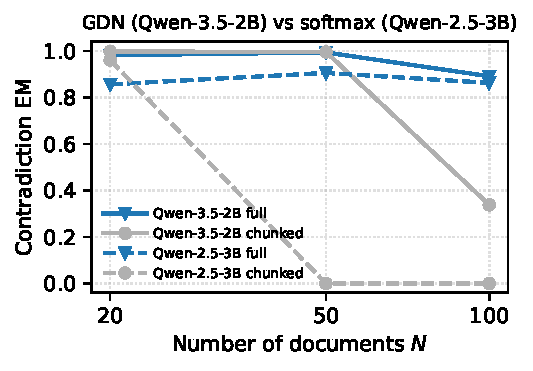
\includegraphics[width=\textwidth]{figures/section4_gdn.pdf}\\
%         \small (a) Qwen-3.5 vs Qwen-2.5
%     \end{minipage}
%     \hfill
%     \begin{minipage}{0.32\textwidth}
%         \centering
%         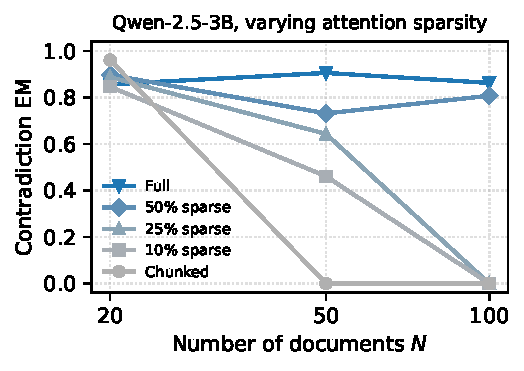
\includegraphics[width=\textwidth]{figures/section4_sparsity.pdf}\\
%         \small (b) Role of sparsity (Qwen-2.5-3B)
%     \end{minipage}
%     \hfill
%     \begin{minipage}{0.32\textwidth}
%         \centering
%         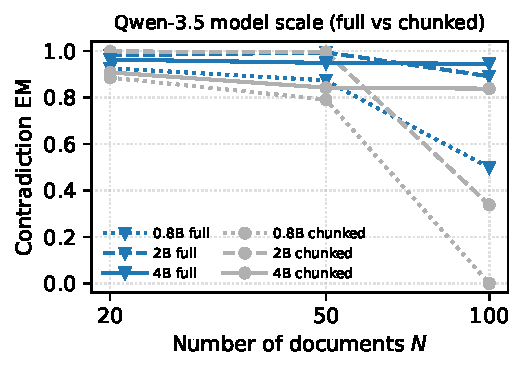
\includegraphics[width=\textwidth]{figures/section4_scale.pdf}\\
%         \small (c) Model scale (Qwen-3.5)
%     \end{minipage}
% \vspace{-0.5em}
% \caption{\textbf{Contradiction-task scaling} \textbf{(a)} Qwen-3.5-2B, with 75\% GDN layers, has better chunked scaling than Qwen-2.5-3B (full attention). \textbf{(b)} Role of attention sparsity: \textbf{greater sparsity leads to faster degradation} with scale.  \textbf{(c)} Increasing model scale within the Qwen-3.5 family (black: 4B, blue: 2B, gray: 0.8B) pushes back the point at which the chunked variant degrades, but \textbf{small full attn models can beat larger chunked attn models}.} 

% \label{fig:sparsityscale}
% \end{figure}



% \amandanote{Not a before-wednesday problem, but we should compare olmo3 7b to olmo3 hybrid 7b to make this argument more cleanly--- they're the same size + data!} \prasannnote{Ohh that's a good idea! }

\textbf{Model Scale Matters Much More For High-\cname} We vary model scale for a few sizes of Qwen-3.5 models (0.8B, 2B, 4B) to examine how model scale affects degradation patterns on four tasks. As shown in Figure~\ref{fig:model_scaling}, once again, while low-\cname tasks seem only minimally affected by model scale, high-\cname tasks show clearer gaps, particularly with chunked attention. \claude{On HotpotQA the relative chunked gap at 32k is $-0.005$, $+0.046$ and $-0.002$ at 0.8B, 2B and 4B --- within noise at every scale, with no ordering. On the high-\cname{} side the gap is large at every scale and moves in opposite directions across the two tasks: on Contradiction it narrows monotonically ($0.396$, $0.353$, $0.261$), while on QDmatch (NQ) it \emph{widens} from $0.729$ at 2B to $0.848$ at 4B. Scaling 5$\times$ therefore closes at most a third of the Contradiction gap and none of the QDmatch gap.} Note that on both high-\cname settings, smaller models with dense attention often outperform larger models with chunked attention. \claude{At 32k the 0.8B model with full attention beats the 4B model with chunked attention on Contradiction ($0.861$ vs.\ $0.699$), and the 2B model with full attention beats 4B-chunked on QDmatch (NQ) by more than 6$\times$ ($0.663$ vs.\ $0.104$).} While not shown here, higher-\cname tasks often have larger minimum model sizes. On Reorder and X-Absence, models under 4B fail to learn, and 0.8B fails to learn on QDmatch (NQ).


\subsection{Analyzing Atomic Operations}

So far, we've largely considered tasks at the \cname class granularity. While this has shown a consistent \emph{relative} trend of architectures and computation not mattering on low-\cname tasks, and mattering greatly on high-\cname tasks, we've not yet said anything about \emph{absolute} values of task difficulty. Recall that our \cname definition assumed a constant average atomic difficulty for tasks as the base unit for complexity. Extending this concept, we posit that tasks with harder atomic task difficulty will be more challenging to scale within complexity class. Likewise, we posit that this difference should compound at higher complexities and with larger corpora.

To test this hypothesis, we start with 4 retrieval tasks varying on a spectrum of difficulty (Contra-NIAH, HotpotQA, NQ, FiQA in ascending order of difficulty), where we difficulty as average performance. We then leverage 4 ``matching'' \ctc{N^2} tasks (QDMatch settings, Contradiction), such that the oracle operation is the same within each task pair (e.g. QDMatch NQ has the same oracle opoeration as NQ). For each task, we then get a measure of how much ``harder'' the \ctc{N^2} version is than the \ctc{N} version by simply looking at the ratio of task-performance at matching context lengths. Note that since retrieval NQ, HotpotQA, and FiQA include hard negatives and the QDmatch settings don't, they're not exactly comparable (hard negatives typically increase retrieval difficulty at lower contexts, and will influence naturally harder tasks like FiQA less).

% ⚠ MOVED, NOT EDITED (no words changed). This wrapfigure sat AFTER the paragraph that cites it,
% with nothing but \begin{figure} floats following it, so there was no running text left to wrap
% around -- wrapfig reported "Stationary wrapfigure forced to float". Placed before that paragraph,
% it now wraps into the text that actually discusses it.
\begin{wrapfigure}{r}{0.5\textwidth}
    \centering
    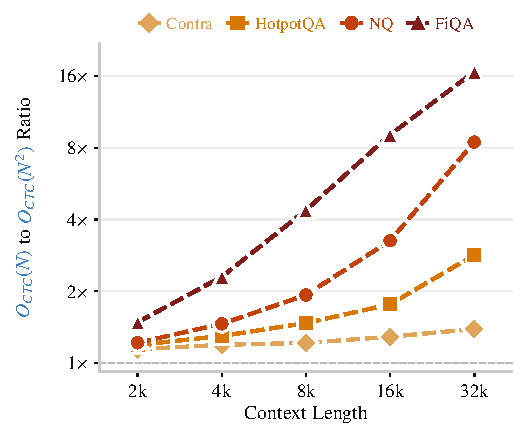
\includegraphics[width=0.48\textwidth]{figures/ctc_qdmatch_compact.pdf}
    \caption{\emph{Oracle Difficulty} For 4 setting pairs (using chunk attention) with matched atomic operations (e.g. NQ vs QDmatch NQ), measure ratio of \claude{\ctc{N} to \ctc{N^2}} task performance\claude{, so 1.0 is parity and higher means the quadratic question has degraded further than the linear one on the same documents}. \textbf{Tasks with harder base operations (darker) see gap grow much faster}}
    \label{fig:atomic_difficulty}
    \vspace{-1em}
\end{wrapfigure}

\paragraph{Tasks With Harder Oracle Difficulty Compound Faster and Predictably} We plot results using chunked attention in Figure~\ref{fig:atomic_difficulty}, the y-axis is \claude{\ctc{N} task performance (e.g.\ NQ) divided by \ctc{N^2} task version performance (e.g.\ QDmatch NQ), so a value of 1.0 means the two versions are equally hard and larger values mean the quadratic version has fallen further behind}. Strikingly, the increase in relative difficulty seems predictable, and strongly supports our \cname hypothesis. \claude{The ordering of the ratios at 32k reproduces the ordering of oracle difficulty exactly: Contra-NIAH/Contradiction $1.39\times$, HotpotQA $2.84\times$, NQ $8.45\times$, FiQA $16.68\times$, against a much tighter $1.14$--$1.48\times$ at 2k. The easiest pair therefore grows its gap by $1.2\times$ across the ladder while the hardest grows it by $11.3\times$.} For the 2 tasks less affected by hard negatives (FiQA, contra), the difficulty increase seems to be in fact linear. \claude{Contradiction rises near-linearly in the plotted (log-spaced) context axis, $1.14 \rightarrow 1.19 \rightarrow 1.21 \rightarrow 1.29 \rightarrow 1.39$, whereas FiQA roughly doubles per rung, $1.48 \rightarrow 2.30 \rightarrow 4.38 \rightarrow 9.07 \rightarrow 16.68$ --- i.e.\ close to linear in the corpus size itself.} This has exciting implications: given knowledge about the atomic operations of a task, and corpus structure, it may be possible to predict ``scaling laws'' for the outcomes of extremely long-context, high-complexity training runs from only small-context, low-complexity training runs. This would be invaluable for long-term development of general corpus reasoning systems.



\begin{figure}[t]
\centering
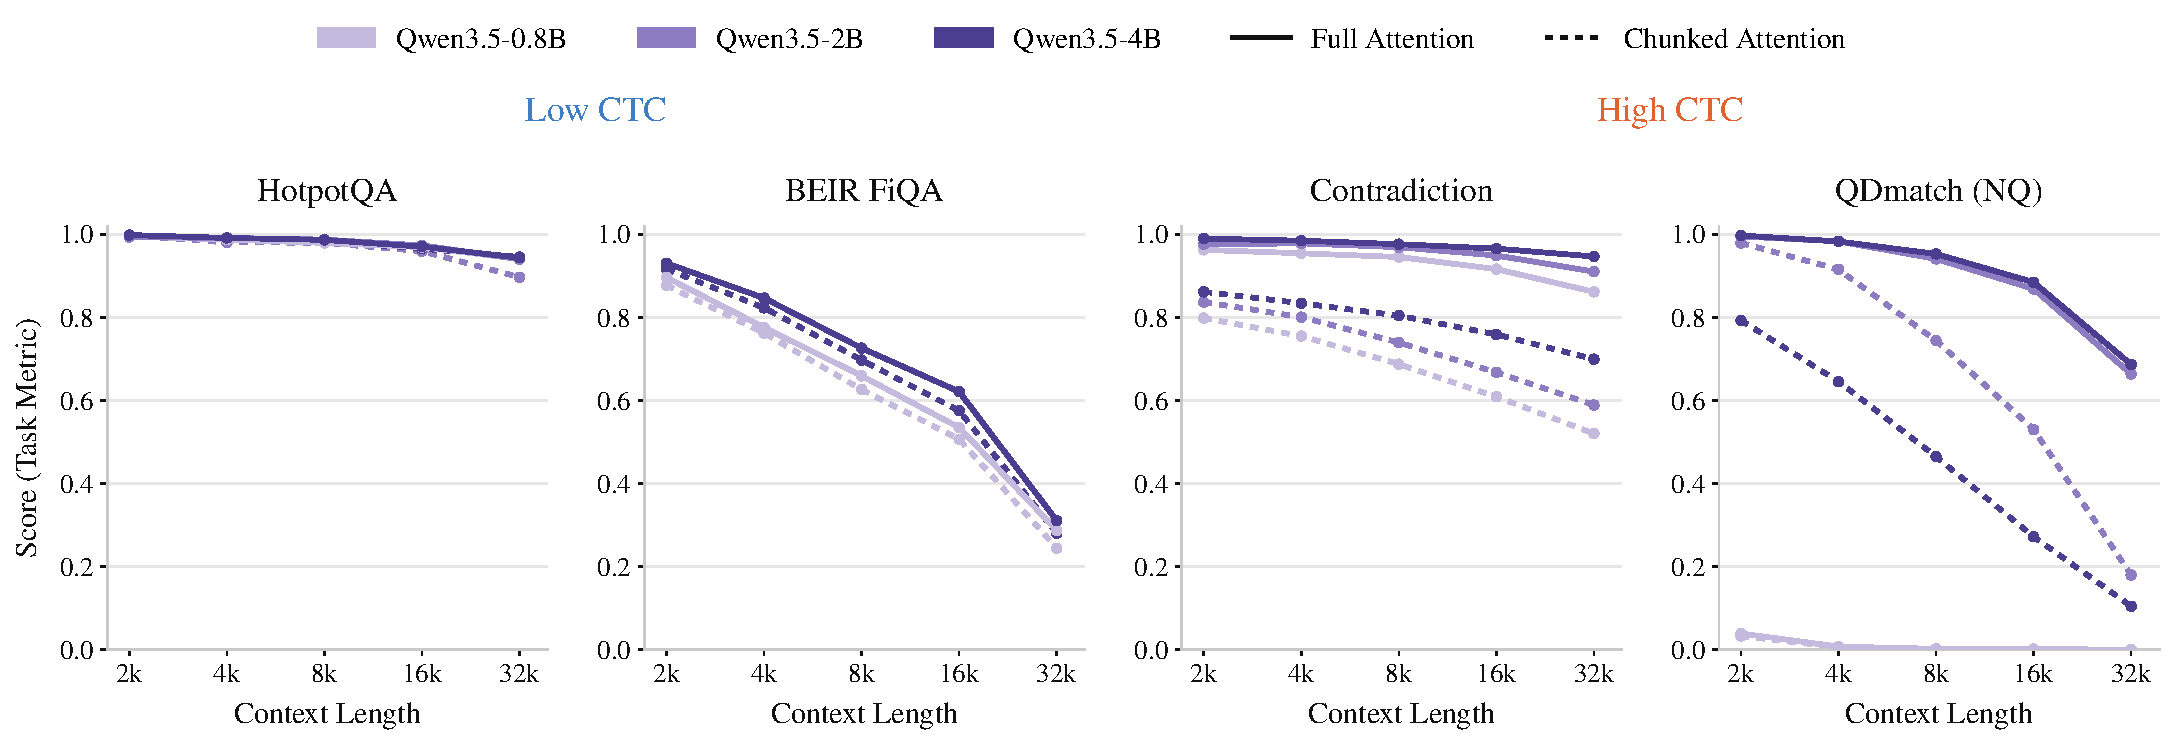
\includegraphics[width=\textwidth]{figures/ctc_scale_row.pdf}
\caption{\emph{Comparing different model scales} We include results for a few different model scales in the Qwen3.5 family. Notably, model scale seems to matter little on low-CTC tasks, but often is important on high-CTC tasks (certain tasks fail when scale is too small. However, there are instances where smaller models with dense attention outperform larger ones with chunked, indicating attention-complexity may be more important past minimal scale).} 
\label{fig:model_scaling}
\end{figure}

% \begin{figure}[t]

%     \centering
%     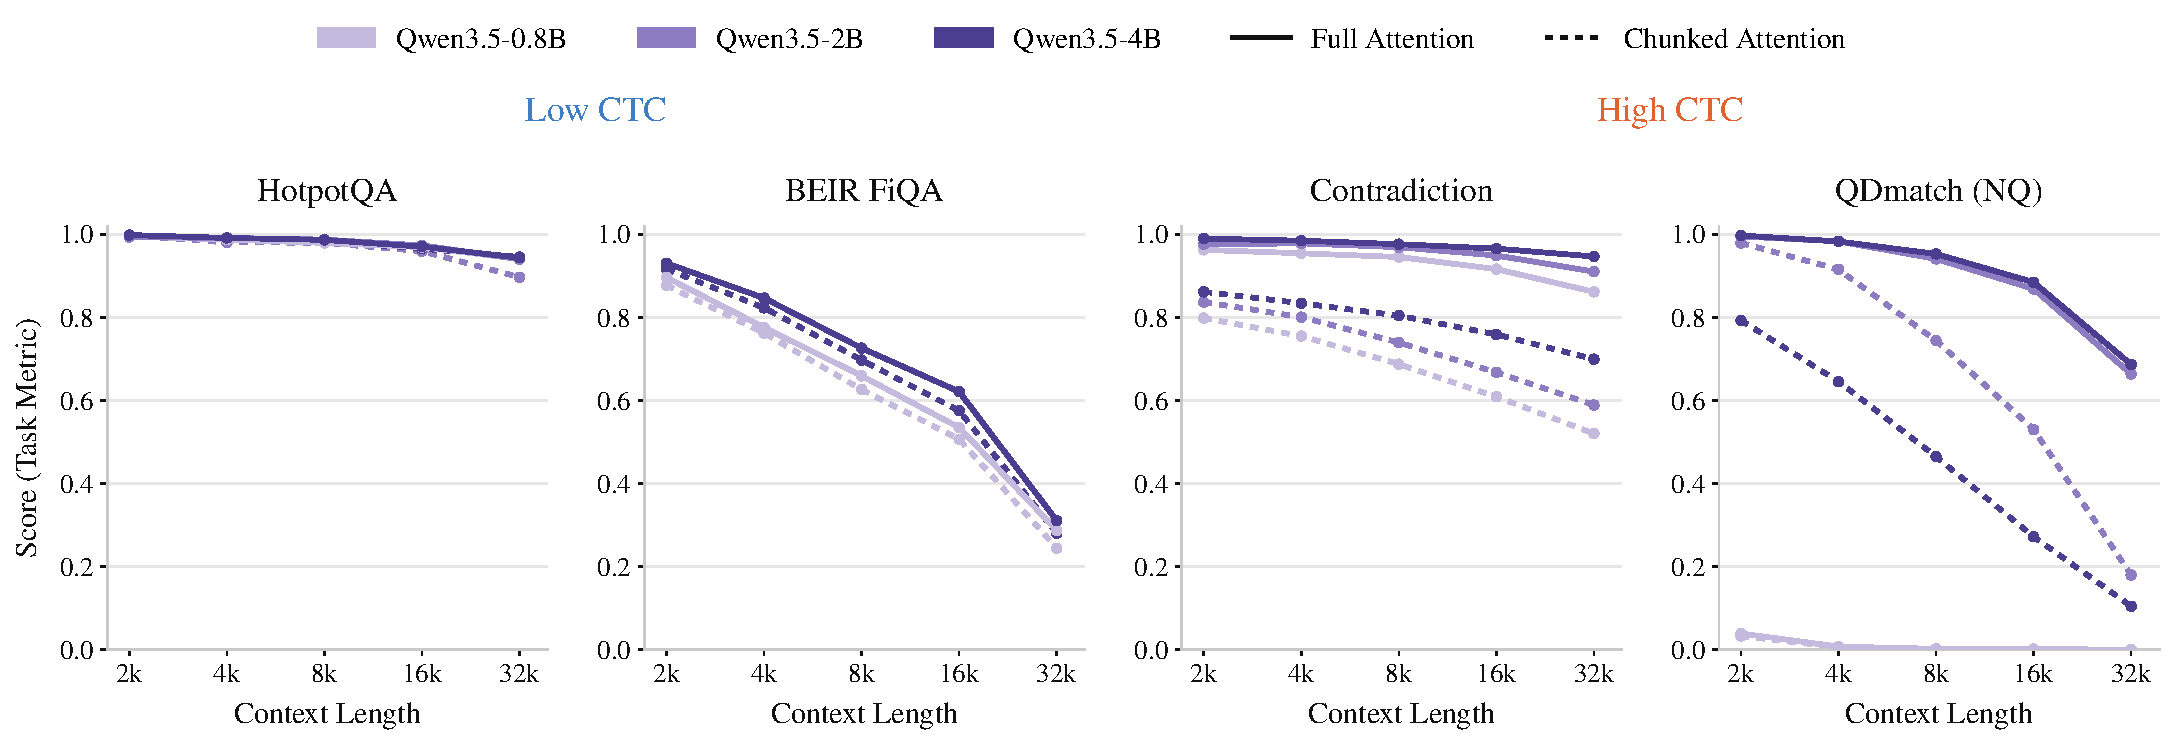
\includegraphics[width=\textwidth]{figures/ctc_scale_row.pdf}
% \caption{\emph{Model scale (Qwen-3.5).} On low-CTC tasks, model scale seems to matter much less, on high-CTC tasks, it can make a large difference, though chunked attention with larger models can be worse than dense attention with smaller ones}

% \label{fig:sparsityscale}

% \end{figure}


% \textbf{Full Attention} Of course, the most expressive approach currently available (full self-attention), is the most expressive, and so in some sense we are bound to tasks which can be reduced to the computational \cmc{N^2} of full attention. The drawback is that this is prohibitively expensive on truly large corpora.

% \textbf{Random Attention Masks} Chunked attention is cheap, but largely forgoes the ability to handle cross-document relationships. One solution is to have each token attend to a random percentage (e.g. 25\%) of prior document tokens (random sparse attention). This is \cmc{N^2}, but with a lower base computation can still be cheaper than full attention.

% \textbf{Chunked Attention} In our simplest chunked attention setting, individual documents can attend within themselves (e.g. Doc 1 content can attend causally to itself, see mask in Figure~TODO), but document tokens can \textbf{not} attend to any other documents. Documents can be encoded cheaply in parallel (thus \cmc{N} computation) but it completely relies on query / cot / answer tokens to handle aggregation and cross-document relations. We implement this via a causal attention mask (see Figure~TODO). 

% \textbf{}{Linear Attention Variants} 

% \paragraph{Random Attention Masks / Anchor Tokens} The above approaches generally lack good ways to build multi-document representations. One potential solution is to have each token attend to a random subset of prior document tokens (random sparse attention), or have dedicated tokens in each document (\emph{anchor tokens}) which all future tokens can attend to, allowing different documents to attend to each other without the cost of full attention, but the overall cross-document attention is much lower, and so these approaches may not learn successfully.



% \prasannnote{We may want to make sure to get good literature coverage. I think we may have it but could be good to confirm}


% \subsection{An Initial Test}

% We evaluate the contradiction task at context size N=20, 50, and 100 with 3 claims, a smaller setting, to get an initial sense of (note in the next section we will examine larger context sizes). Based on some iteration (TODO Appendix), we compare the case of both using a chain of thought which heavily enumerates all documents, and a no-CoT case. We evaluate various attention mechanisms, from chunked to full attention, at varying levels of sparsity (e.g. random, document window sparsity at 5, 25, and 50 percent). Note that retrieval baseline performance on this task is inherently random.

% \paragraph{Results} We plot sparsity of different approaches and models vs performance on the task in Figure~TODO (note that all of these were trained and evaluated on the same in-domain data). We find that without the CoT, even at the 20 claim scale (500 tokens), models struggle to learn this task well without full attention. \prasann{TODO get / put in more results in between pure chunked and full attn}. With the CoT, things are a bit better, but standard attention seems to improve similarly if not more than sparse variants as a function of the sparsity. \prasann{One potential risk is that "you just haven't trained on enough data to overcome OODness of new attention mask", so we should probably select 1-2 runs to run at really large scale to sanity check this (though I think from looking at the loss curves I think we should be fine here)}

% Overall, in particular when taking in the relationship between model scale and various attention types that we examine, we conclude that there seems to be a relationship between how much computation different approaches provide, and the corresponding performance. \prasann{Hmm I wonder if there's a single "computation" number which we could plot and get a clean performance line for within model family...}